\documentclass[aspectratio=169,11pt]{beamer}

\usepackage{fontspec}
\setsansfont{DejaVu Sans}
\setmonofont{DejaVu Sans Mono}
\usepackage[polish]{babel}
\usepackage{amsmath,amssymb,bm}
\usepackage{graphicx}
\usepackage{booktabs}
\usepackage{tikz}
\usetikzlibrary{arrows.meta,positioning,calc,fit,shapes.geometric}
\usepackage{hyperref}
\usepackage{listings}
\usepackage{pgfpages}

\hypersetup{colorlinks=true, urlcolor=blue!70!black, linkcolor=blue!70!black}
\setbeameroption{hide notes}
\setbeamertemplate{navigation symbols}{}
\setbeamertemplate{footline}{%
  \leavevmode\hbox{%
  \begin{beamercolorbox}[wd=.78\paperwidth,ht=2.7ex,dp=1ex,leftskip=1em]{author in head/foot}%
    MPC dla robota kroczącego: od jednej nogi do architektury bezpieczeństwa
  \end{beamercolorbox}%
  \begin{beamercolorbox}[wd=.22\paperwidth,ht=2.7ex,dp=1ex,center]{date in head/foot}%
    \insertframenumber/\inserttotalframenumber
  \end{beamercolorbox}}%
}
\setbeamertemplate{itemize item}{\raisebox{0.15ex}{\scriptsize$\blacktriangleright$}}
\setbeamertemplate{itemize subitem}{\scriptsize$\circ$}
\setbeamersize{text margin left=9mm,text margin right=9mm}

\definecolor{pwrblue}{RGB}{22,74,132}
\definecolor{darktext}{RGB}{25,25,25}
\definecolor{softgray}{RGB}{245,247,250}
\definecolor{warn}{RGB}{160,65,25}
\definecolor{safe}{RGB}{34,120,70}
\setbeamercolor{title}{fg=pwrblue}
\setbeamercolor{frametitle}{fg=pwrblue}
\setbeamercolor{normal text}{fg=darktext}
\setbeamercolor{block title}{fg=white,bg=pwrblue}
\setbeamercolor{block body}{fg=darktext,bg=softgray}

\lstdefinestyle{pseudocode}{
  basicstyle=\ttfamily\small,
  columns=fullflexible,
  keepspaces=true,
  showstringspaces=false,
  frame=single,
  rulecolor=\color{black!20},
  backgroundcolor=\color{softgray}
}

\newcommand{\source}[1]{{\vfill\tiny\color{black!55}Źródło / kontekst: #1}}
\newcommand{\key}[1]{\textbf{\color{pwrblue}#1}}
\newcommand{\warntext}[1]{\textbf{\color{warn}#1}}
\newcommand{\safetext}[1]{\textbf{\color{safe}#1}}

\title{Model Predictive Control dla czworonożnego robota kroczącego}
\subtitle{Od regulacji punkt--punkt jednej nogi do bezpiecznej architektury sterowania}
\author{Łukasz Janiec}
\date{2026}

\begin{document}

% 1
\begin{frame}[plain]
  \titlepage
  \vspace{-1.2em}
  \begin{center}
  \small Dla inżynierów: jasno, ale bez ukrywania modelu, ograniczeń i ryzyk.
  \end{center}
  \note{Slajd ustawia cel prezentacji: nie jest to gotowa obietnica produktu, tylko początek projektu badawczego nad sterowaniem predykcyjnym i bezpieczeństwem lokomocji.}
\end{frame}

% 2
\begin{frame}{Cel projektu w jednym obrazie}
\begin{columns}[T,onlytextwidth]
\column{0.56\textwidth}
\begin{itemize}
  \item Mamy czworonożnego robota z nietypową nogą opartą o mechanizm czworoboku.
  \item Obecne sterowanie oparte na \key{Reinforcement Learning}, czyli uczeniu przez wzmacnianie, działa w wielu próbach.
  \item Problem: polityka może wprowadzić robota w konfiguracje trudne do odzyskania na realnym podłożu.
  \item Hipoteza projektu: \key{model + predykcja + bariery bezpieczeństwa} mogą zmniejszyć liczbę takich awarii.
\end{itemize}
\column{0.40\textwidth}
\begin{center}
\begin{tikzpicture}[scale=0.88,>=Latex]
  \draw[thick,rounded corners=3pt,fill=blue!8] (-1.7,0.25) rectangle (1.7,1.05);
  \node[font=\small] at (0,0.65) {korpus robota};
  \foreach \x/\d in {-1.25/-1,-0.45/1,0.45/-1,1.25/1} {
    \draw[very thick] (\x,0.25)--(\x+0.25*\d,-0.65)--(\x+0.55*\d,-1.35);
    \fill[safe] (\x+0.55*\d,-1.40) circle (0.07);
  }
  \draw[->,thick,pwrblue] (-1.9,1.4)--(1.9,1.4);
  \node[font=\scriptsize] at (0,1.65) {ruch korpusu i harmonogram kontaktów};
  \node[font=\scriptsize,align=center] at (0,-1.95) {RL proponuje ruch\\MPC i CBF kontrolują ryzyko};
\end{tikzpicture}
\end{center}

Czym jest MPC: przewidywanie, optymalizacja, ograniczenia, sterowanie w pętli.
\end{columns}
\source{Opis platformy z KKR: cztery kończyny, 3 stopnie swobody na kończynę, ROS 2, CAN, tryby sterowania napędów.}
\note{Należy wyjaśnić, że projekt nie neguje uczenia przez wzmacnianie. Chodzi o dodanie warstwy modelowej i bezpieczeństwa tam, gdzie czysta polityka uczona nie ma jawnych gwarancji.}
\end{frame}

% 3
\begin{frame}{Platforma: co wiemy z dokumentacji}
\begin{itemize}
  \item Korpus aluminiowy i cztery kończyny.
  \item Każda kończyna: \key{trzy stopnie swobody}.
  \item Główna część nogi: mechanizm czworoboku przegubowego / równoległoboku.
  \item Napędy: silniki bezszczotkowe prądu stałego z przekładniami planetarnymi.
  \item Sterowanie z komputera przez \key{Robot Operating System 2 (ROS 2)} i \key{Controller Area Network (CAN)}.
\end{itemize}
{\vspace{0.15em}\tiny\color{black!55}Źródło: załączony PDF, s. 1-2. Pełne dane CAD, bezwładności i ograniczenia momentu wymagają uzupełnienia.}
\note{Tu trzeba wyraźnie odróżnić fakty z PDF-a od przyszłych założeń modelowych. Dokładny model wymaga CAD-u, danych silników, przekładni i identyfikacji.}
\end{frame}

% 4
\begin{frame}{Dlaczego to nie jest „zwykły manipulator na nogach”?}
\begin{columns}[T,onlytextwidth]
\column{0.52\textwidth}
\begin{itemize}
  \item Robot kroczący zmienia punkty kontaktu z podłożem.
  \item Kontakt może się pojawić, zniknąć, poślizgnąć albo uderzyć w podłoże.
  \item Tarcie i nierówności podłoża są częścią sterowania, nie tylko zakłóceniem.
  \item Błąd jednej nogi może zmienić równowagę całego korpusu.
  \item Kontakt i podłoże są aktywnymi elementami układu.
\end{itemize}
\column{0.44\textwidth}
\begin{block}{Konsekwencja dla sterowania}
Sterownik musi planować ruch, siły i bezpieczeństwo konfiguracji, a nie tylko śledzić zadaną trajektorię przegubów.
\end{block}
\vspace{0.5em}
\begin{center}
\begin{tikzpicture}[scale=0.9]
  \draw[thick,rounded corners=2pt,fill=blue!6] (-1.5,0.2) rectangle (1.5,0.8);
  \foreach \x/\s in {-1.2/1, -0.45/0, 0.45/1, 1.2/0} {
    \draw[thick] (\x,0.2) -- (\x-0.25,-0.8);
    \draw[thick] (\x,0.2) -- (\x+0.25,-0.8);
    \ifnum\s=1 \fill[safe] (\x,-0.85) circle (0.08); \else \draw[warn,thick] (\x,-0.85) circle (0.08); \fi
  }
  \draw[black!40,thick] (-2,-0.95) -- (2,-0.95);
  \node[align=center,font=\scriptsize] at (0,-1.35) {kontakt aktywny / noga w przenoszeniu};
\end{tikzpicture}
\end{center}
\end{columns}
\note{To dobry slajd dla laików: kontakt i podłoże są aktywnymi elementami układu. W sterowaniu manipulatorów zwykle mamy stałą podstawę, a tutaj podstawa musi być utrzymywana przez same nogi.}
\end{frame}

% 5
\begin{frame}{Obecny punkt startowy: uczenie przez wzmacnianie}
\small
\begin{columns}[T,onlytextwidth]
\column{0.49\textwidth}
\begin{block}{Reinforcement Learning (RL)}
Polityka sterowania uczona przez próby i nagrody w symulacji lub na robocie.
\end{block}
\begin{itemize}
  \item Znajduje złożone zachowania bez ręcznego programowania każdego kroku.
  \item Po treningu działa szybko.
  \item Bezpieczeństwo bywa zapisane tylko pośrednio w funkcji nagrody.
\end{itemize}
\column{0.47\textwidth}
\begin{center}
\begin{tikzpicture}[node distance=0.65cm,>=Latex]
  \tikzstyle{box}=[draw,rounded corners=2pt,fill=blue!6,minimum width=3.0cm,minimum height=0.72cm,align=center,font=\small]
  \node[box] (obs) {obserwacje\\czujników};
  \node[box,below=of obs] (policy) {polityka RL};
  \node[box,below=of policy] (cmd) {zadane pozycje\\lub momenty};
  \node[box,below=of cmd] (robot) {robot + podłoże};
  \draw[->,thick] (obs) -- (policy);
  \draw[->,thick] (policy) -- (cmd);
  \draw[->,thick] (cmd) -- (robot);
  \draw[->,thick] (robot.west) .. controls +(-1.0,0) and +(-1.0,0) .. (obs.west);
\end{tikzpicture}
\end{center}
\end{columns}
\note{Należy podkreślić, że RL jest mocnym punktem startowym. Problemem nie jest brak ruchu, tylko brak jawnego mechanizmu wykluczania stanów niebezpiecznych lub nieodzyskiwalnych.}
\end{frame}

% 6
\begin{frame}{Awaria, która motywuje projekt}
\begin{columns}[T,onlytextwidth]
\column{0.52\textwidth}
\begin{itemize}
  \item Przykład: nogi ustawiają się zbyt szeroko na boki.
  \item Na szorstkim podłożu stopa nie przesuwa się łatwo do środka.
  \item Napęd może mieć za mały zapas momentu, aby odzyskać postawę.
  \item Polityka działała lokalnie sensownie, ale weszła w obszar o złej geometrii i złym kontakcie.
\end{itemize}
\column{0.44\textwidth}
\begin{block}{Nie chodzi tylko o „lepszy trening”}
Potrzebujemy wykryć i opisać zbiór konfiguracji, do których sterownik nie powinien dopuszczać.
\end{block}
\vspace{0.2em}
\begin{center}
\begin{tikzpicture}[scale=0.82]
 \draw[thick,fill=blue!5] (-1.1,0.3) rectangle (1.1,0.75);
 \foreach \x/\dx in {-0.8/-0.85,0.8/0.85} {
   \draw[ultra thick] (\x,0.3)--(\x+\dx,-0.75);
   \draw[ultra thick] (\x+\dx,-0.75)--(\x+1.25*\dx,-1.35);
   \fill[warn] (\x+1.25*\dx,-1.40) circle (0.08);
 }
 \draw[black!40,thick] (-2.3,-1.5)--(2.3,-1.5);
 \node[font=\scriptsize,align=center] at (0,-1.85) {duży rozstaw + tarcie = trudny powrót};
\end{tikzpicture}
\end{center}
\end{columns}
\note{Slajd ma przełożyć intuicję użytkownika na problem sterowania: niepożądana konfiguracja może wynikać z połączenia geometrii, tarcia, momentu i braku planowania odzysku.}
\end{frame}

% 7
\begin{frame}{Jedna noga jako pierwszy model badawczy}
\begin{columns}[T,onlytextwidth]
\column{0.50\textwidth}
\begin{itemize}
  \item Pełny robot jest trudny: wiele kontaktów, całe ciało, stabilność, opóźnienia.
  \item Jedna noga jest mniejszym, ale nadal wartościowym problemem.
  \item Możemy badać: geometrię, osobliwości, momenty, tarcie i bezpieczne zakresy ruchu.
\end{itemize}
\column{0.46\textwidth}
\begin{center}
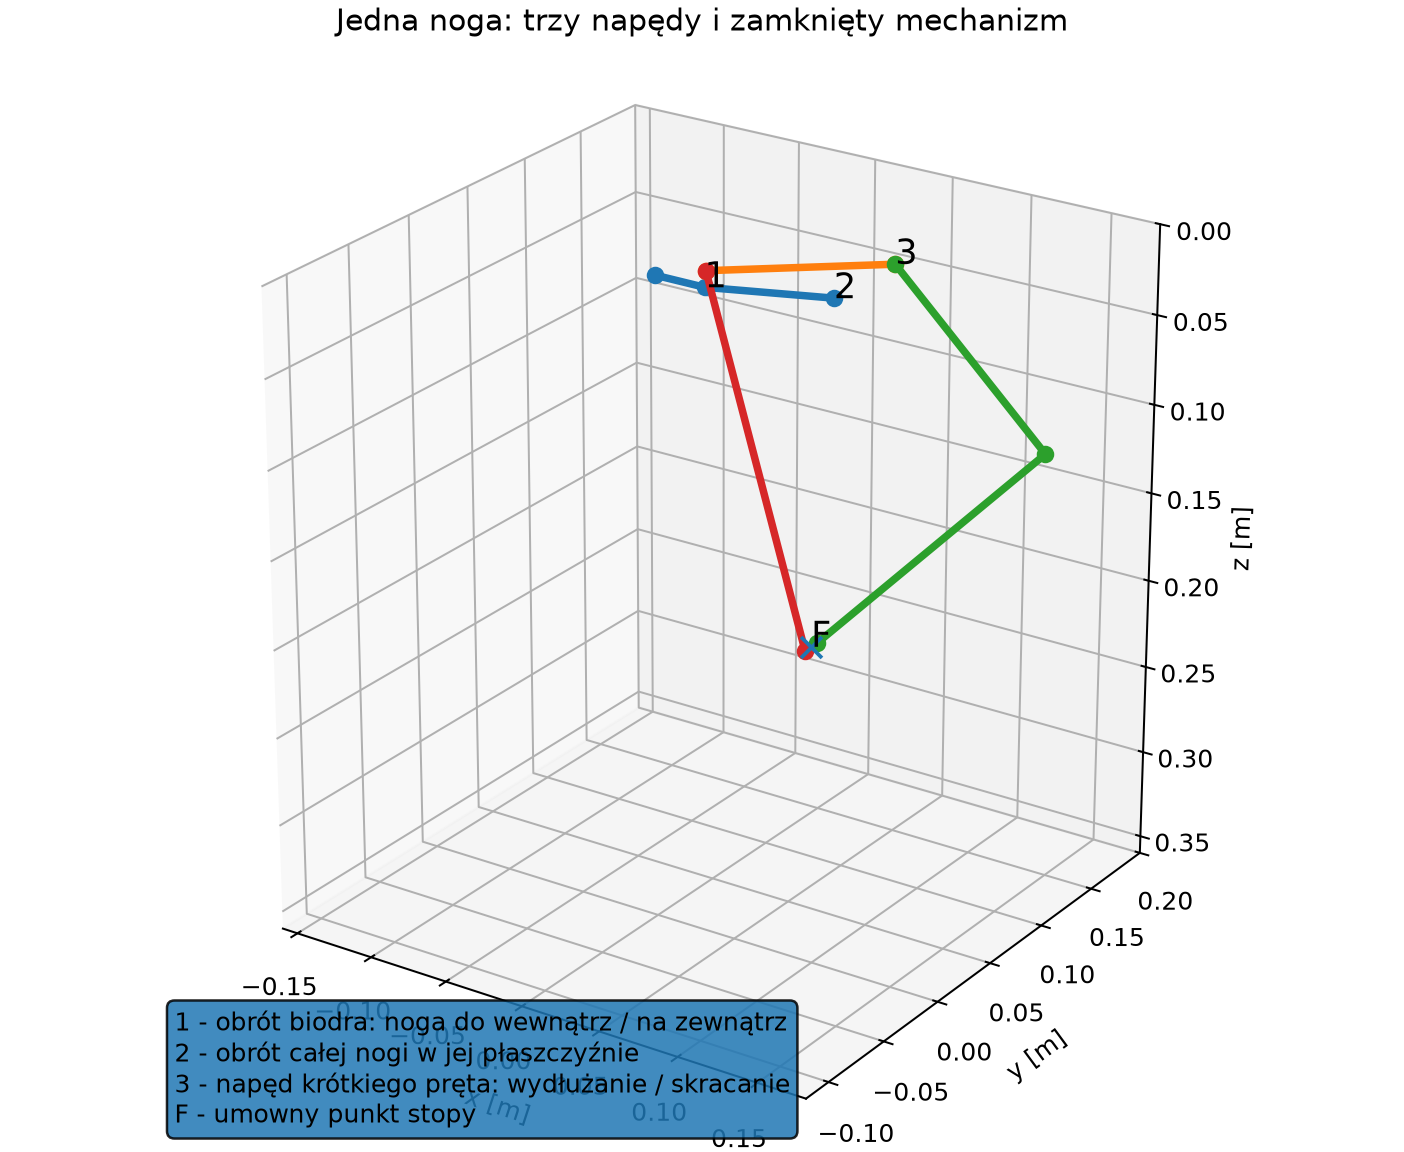
\includegraphics[width=0.9\linewidth,height=0.48\textheight,keepaspectratio]{figures/leg_three_motor_roles_annotated.png}
\end{center}
\end{columns}
\begin{block}{Minimalny cel demonstratora jednej nogi}
Przesunąć stopę do celu, ale nie wejść w konfigurację, z której noga nie może wrócić przy realistycznym tarciu i ograniczonych momentach.
\end{block}
\note{To jest kluczowa zmiana względem wersji z odwróconym wahadłem. Przykład jednej nogi jest bliższy platformie i może być pierwszym niezależnym pakietem badawczym.}
\end{frame}

% 8
\begin{frame}{Trzy napędy jednej nogi: poprawna interpretacja}
\begin{columns}[T,onlytextwidth]
\column{0.56\textwidth}
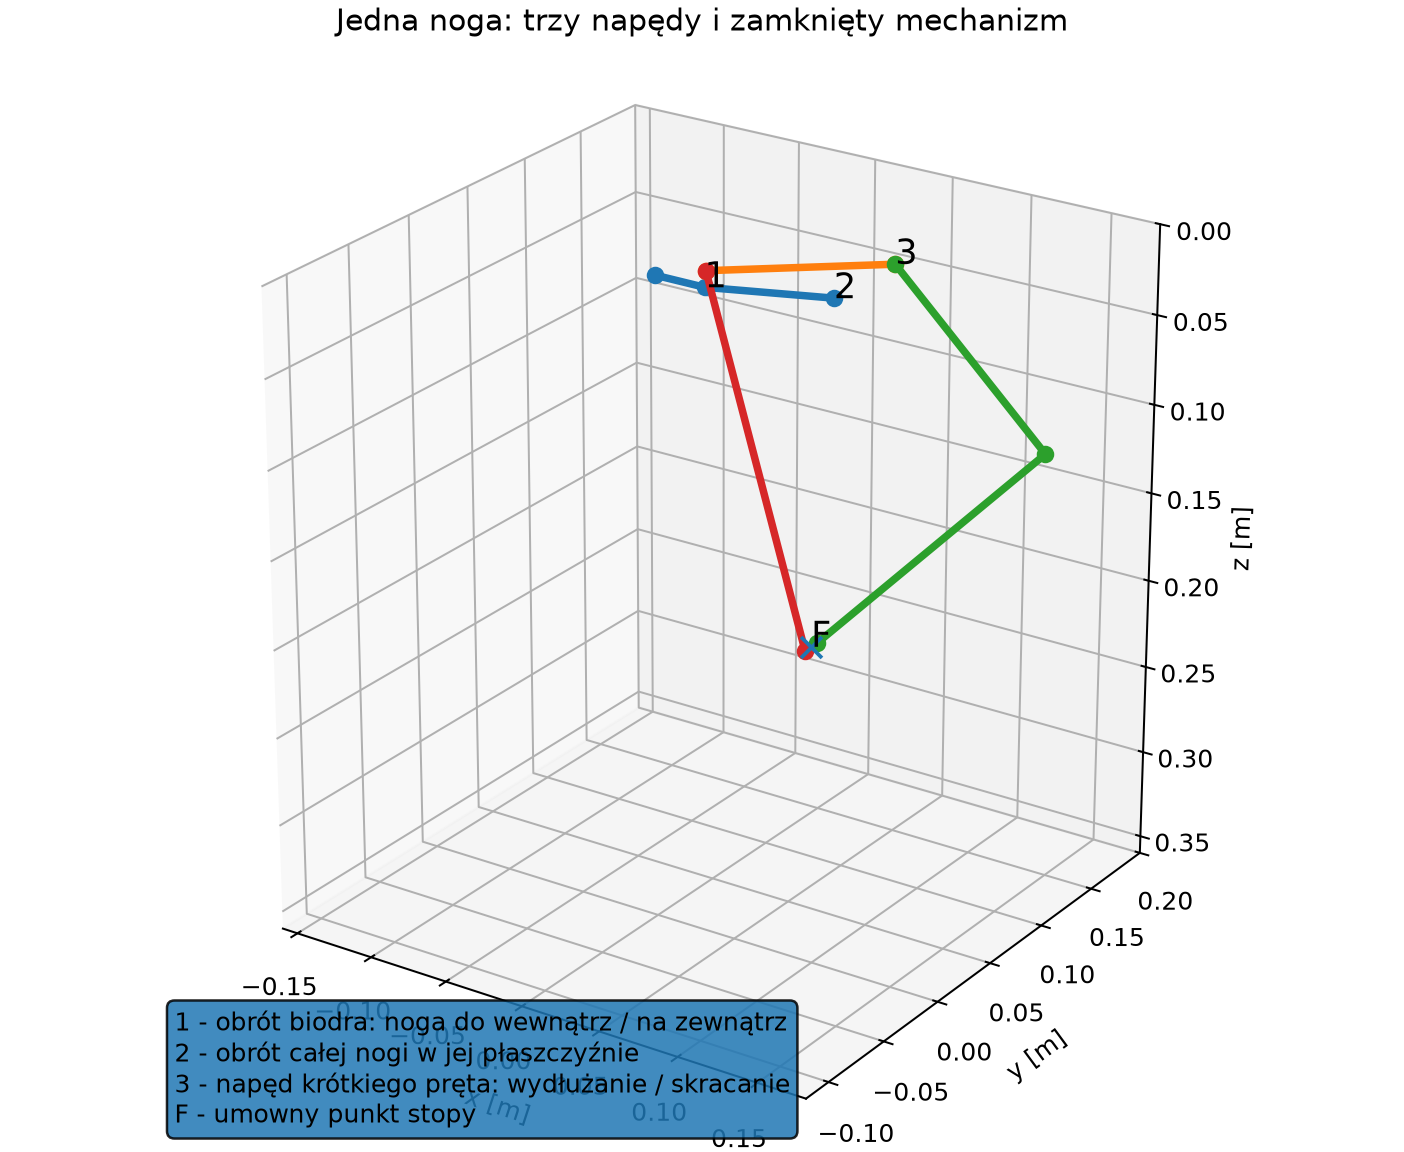
\includegraphics[width=\linewidth,height=0.66\textheight,keepaspectratio]{figures/leg_three_motor_roles_annotated.png}
\column{0.40\textwidth}
\small
\begin{itemize}
  \item $q_{\mathrm{hip}}$: silnik prostopadły do płaszczyzny nogi; ruch biodra do wewnątrz i na zewnątrz od korpusu.
  \item $q_{\mathrm{sweep}}$: obrót całej nogi zgodnie lub przeciwnie do ruchu wskazówek zegara.
  \item $q_{\mathrm{extend}}$: obrót jednego krótkiego pręta czworoboku; zmiana geometrii wydłuża lub skraca nogę.
  \item Dwa pozostałe kąty pętli są bierne i wynikają z jej domknięcia.
\end{itemize}
\end{columns}
\source{Model URDF i kod kinematyki w repozytorium \href{https://github.com/delipl/quadruped_ros2}{delipl/quadruped\_ros2}.}
\note{Poprzedni opis sugerował zbyt ogólnie trzy niezależne przeguby. Tutaj trzeba jasno rozróżnić ruch biodra, obrót całej płaszczyzny nogi oraz napęd krótkiego pręta zamkniętego mechanizmu.}
\end{frame}

% 9
\begin{frame}{Mechanizm czteroprętowy: napęd i kąty bierne}
\begin{columns}[T,onlytextwidth]
\column{0.54\textwidth}
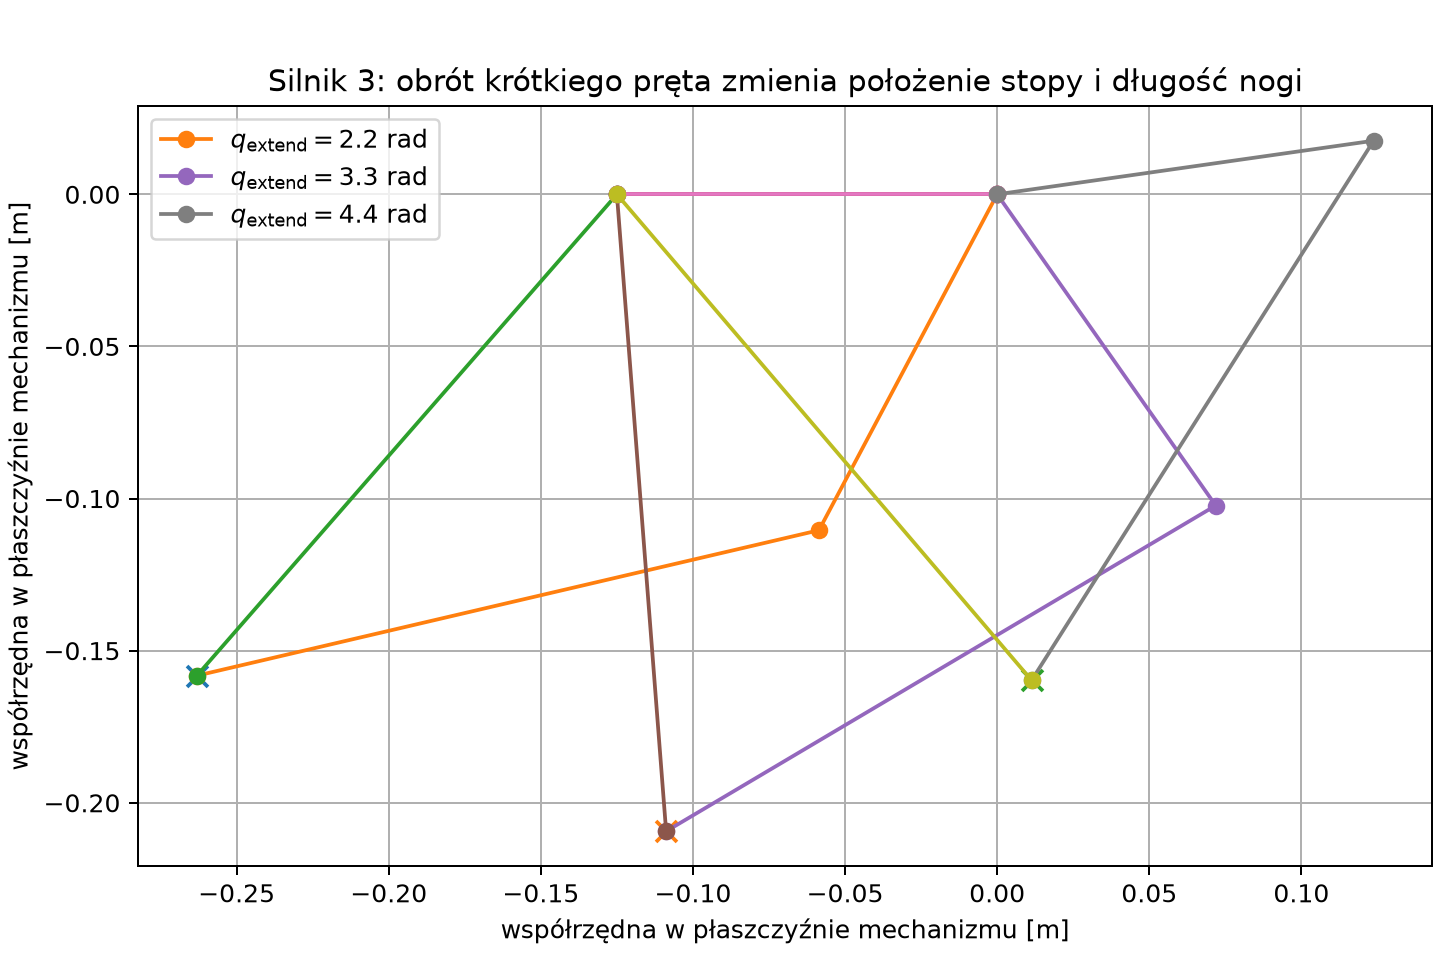
\includegraphics[width=\linewidth,height=0.63\textheight,keepaspectratio]{figures/four_bar_extension_side_view.png}
\column{0.42\textwidth}
\begin{block}{Współrzędne aktywne}
\[
q_a = \begin{bmatrix}
q_{\mathrm{hip}} & q_{\mathrm{sweep}} & q_{\mathrm{extend}}
\end{bmatrix}^{T}
\]
\end{block}
\begin{block}{Domknięcie pętli}
\[
q_p=g(q_{\mathrm{extend}}),
\qquad \Phi(q_a,q_p)=0.
\]
\end{block}
\end{columns}
\note{W kodzie Pythona dwa kąty bierne są rekonstruowane przez bezpośrednią adaptację funkcji update_passive_joints z kontrolera ROS 2.}
\end{frame}

% 10
\begin{frame}{Kinematyka: gdzie jest stopa i jak szybko się porusza?}
\begin{columns}[T,onlytextwidth]
\column{0.50\textwidth}
\begin{block}{Położenie stopy}
\[
p_F = f_{\mathrm{kin}}(q)
\]
\end{block}
\begin{block}{Prędkość stopy}
\[
\dot p_F = J(q)\dot q
\]
\end{block}
\column{0.46\textwidth}
\begin{itemize}
  \item $p_F$ - położenie stopy w układzie robota.
  \item $J(q)$ - macierz Jacobiego: lokalne przełożenie prędkości przegubów na prędkość stopy.
  \item W praktyce $J(q)$ mówi też, czy ruch jest dobrze uwarunkowany.
\end{itemize}
\vspace{0.4em}
\begin{center}
\begin{tikzpicture}[>=Latex,scale=0.95]
  \draw[thick,fill=blue!5] (0,0) circle (0.18);
  \draw[ultra thick] (0,0)--(1.2,-0.8)--(2.1,-1.65);
  \fill[safe] (2.1,-1.65) circle (0.08);
  \draw[->,thick,pwrblue] (2.1,-1.65)--(2.75,-1.25);
  \node[font=\scriptsize] at (2.95,-1.12) {$\dot p_F$};
  \draw[->,thick,warn] (0.25,0.05) arc (10:-50:0.5);
  \node[font=\scriptsize] at (0.8,0.1) {$\dot q$};
\end{tikzpicture}
\end{center}
\end{columns}
\note{To jeden z najważniejszych slajdów edukacyjnych: laik inżynier widzi, że macierz Jacobiego nie jest abstrakcją, tylko lokalnym przełożeniem ruchu napędów na ruch stopy.}
\end{frame}

% 11
\begin{frame}{Osobliwości i utrata „sprawczości” nogi}
\small
\begin{columns}[T,onlytextwidth]
\column{0.52\textwidth}
\begin{itemize}
  \item W dobrej konfiguracji mały ruch napędu daje kontrolowany ruch stopy.
  \item W złej konfiguracji stopa może prawie nie reagować albo wymagać dużego momentu.
  \item W mechanizmach równoległych dochodzą granice geometrii i możliwe złe gałęzie ruchu.
\end{itemize}
\begin{block}{Przykładowy margines}
\vspace{-0.7em}
\[
h_{\mathrm{sing}}(q) = \sigma_{\min}(J(q)) - \varepsilon \ge 0
\]
\vspace{-1.0em}
\end{block}
\column{0.44\textwidth}
\begin{center}
\begin{tikzpicture}[scale=0.82]
  \draw[->] (-0.2,0)--(4.0,0) node[right,font=\scriptsize] {konfiguracja};
  \draw[->] (0,-0.2)--(0,2.1) node[above,font=\scriptsize] {margines};
  \draw[thick,safe] plot[smooth] coordinates {(0.2,1.8)(1.0,1.6)(1.8,1.1)(2.6,0.45)(3.4,0.12)};
  \draw[thick,warn,dashed] (0,0.45)--(3.8,0.45);
  \node[font=\scriptsize,align=center] at (2.5,1.35) {bezpiecznie};
  \node[font=\scriptsize,align=center,warn] at (2.8,0.25) {za blisko\\osobliwości};
\end{tikzpicture}
\end{center}
\begin{itemize}
  \item Dla realnej nogi margines może łączyć geometrię, tarcie i zapas momentu.
\end{itemize}
\end{columns}
\note{Warto powiedzieć, że formuła z minimalną wartością osobliwą Jacobiego jest przykładem. Dla rzeczywistej nogi może być potrzebny lepszy margines: zapas momentu, odległość od limitów, lub miara odzyskiwalności.}
\end{frame}

% 12
\begin{frame}{Dynamika nogi i kontakt z podłożem}
\begin{block}{Ogólny model dynamiki}
\[
M(q)\ddot q + C(q,\dot q)\dot q + g(q) = B\tau + J_c(q)^T f_c
\]
\end{block}
\begin{columns}[T,onlytextwidth]
\column{0.48\textwidth}
\begin{itemize}
  \item $M(q)$ - bezwładność.
  \item $C(q,\dot q)\dot q$ - efekty zależne od prędkości.
  \item $g(q)$ - grawitacja.
\end{itemize}
\column{0.48\textwidth}
\begin{itemize}
  \item $\tau$ - momenty napędów.
  \item $f_c$ - siły kontaktu stopy z podłożem.
  \item $J_c(q)^T f_c$ - przełożenie sił kontaktu na przeguby.
\end{itemize}
\end{columns}
\begin{block}{Poziom dokładności}
Dokładny model jest potrzebny do walidacji; model sterowania czasu rzeczywistego może być uproszczony, ale musi zachować kluczowe ograniczenia.
\end{block}
\note{To nie ma być wykład z mechaniki analitycznej. Slajd ma pokazać, które zjawiska trzeba uwzględnić, kiedy z pozycji stopy przechodzimy do momentów silników i realnego kontaktu.}
\end{frame}

% 13
\begin{frame}{Sterowanie impedancyjne napędu}
\begin{columns}[T,onlytextwidth]
\column{0.56\textwidth}
\begin{block}{Idea: wirtualna sprężyna i tłumik}
\[
\tau = K_p(q_d-q) + K_d(\dot q_d-\dot q) + \tau_{\mathrm{ff}}
\]
\end{block}
\begin{itemize}
  \item $K_p$ - wzmocnienie części proporcjonalnej: „sztywność”.
  \item $K_d$ - wzmocnienie części zależnej od prędkości: „tłumienie”.
  \item $\tau_{\mathrm{ff}}$ - moment wyprzedzający, zadany z wyższego poziomu sterowania.
\end{itemize}
\column{0.40\textwidth}
\begin{center}
\begin{tikzpicture}[node distance=0.55cm,>=Latex]
  \tikzstyle{box}=[draw,rounded corners=2pt,fill=blue!6,minimum width=2.8cm,minimum height=0.65cm,align=center,font=\scriptsize]
  \node[box] (ref) {pozycja i prędkość\\zadana};
  \node[box,below=of ref] (law) {$K_p e_q + K_d e_{\dot q}$\\$+\;\tau_{\mathrm{ff}}$};
  \node[box,below=of law] (motor) {sterownik prądu\\i silnik};
  \node[box,below=of motor] (enc) {enkoder};
  \draw[->,thick] (ref)--(law);
  \draw[->,thick] (law)--node[right,font=\scriptsize] {$\tau$} (motor);
  \draw[->,thick] (motor)--(enc);
  \draw[->,thick] (enc.west) .. controls +(-0.9,0) and +(-0.9,0) .. (law.west);
\end{tikzpicture}
\end{center}
\end{columns}
\source{Załączony PDF wskazuje tryb impedancyjny sterowników napędów oraz komunikację ROS 2/CAN.}
\note{Ten slajd buduje most do sprzętu: wyższa warstwa nie musi zawsze wysyłać surowych momentów. Może zadawać pozycje, prędkości, sztywności i feed-forward, jeśli sterownik napędu to obsługuje.}
\end{frame}

% 14
\begin{frame}[fragile]{„Model” w praktyce: interfejs, nie dogmat}
\begin{columns}[T,onlytextwidth]
\column{0.51\textwidth}
\begin{lstlisting}[style=pseudocode,basicstyle=\ttfamily\scriptsize]
state = read_sensors()
q  = state.joint_position
dq = state.joint_velocity

foot = model.foot_position(q)
J    = model.foot_jacobian(q)
h    = model.safety_margins(q, dq)
\end{lstlisting}
\column{0.45\textwidth}
\small
\begin{itemize}
  \item Model może być analityczny, numeryczny lub częściowo zidentyfikowany.
  \item Najważniejsze pytanie: \key{czy przewiduje właściwe ryzyka?}
  \item Na początku wystarczą kinematyka, ograniczenia, margines osobliwości i prosta dynamika.
\end{itemize}
\end{columns}
\note{To dobry slajd do rozbrojenia obawy, że model musi być idealny. Sterowanie predykcyjne potrzebuje modelu użytecznego dla horyzontu predykcji, nie kompletnego cyfrowego bliźniaka.}
\end{frame}

% 15
\begin{frame}{MPC: Model Predictive Control w jednym zdaniu}
\begin{block}{Definicja robocza}
\key{Model Predictive Control (MPC)}, czyli sterowanie predykcyjne oparte na modelu, wybiera teraz takie sterowanie, które według modelu da najlepszy i bezpieczny ruch w najbliższej przyszłości.
\end{block}
\vspace{-0.2em}
\[
\begin{aligned}
\min_{u_0,\ldots,u_{N-1}}\quad
&\sum_{k=0}^{N-1} \ell(x_k,u_k)+\ell_N(x_N)\\
\text{przy ograniczeniach}\quad
&x_{k+1}=f(x_k,u_k),\\
&x_k\in\mathcal X,\qquad u_k\in\mathcal U.
\end{aligned}
\]
\begin{itemize}
  \item $x_k$ - przewidywany stan, $u_k$ - sterowanie, $N$ - horyzont predykcji.
  \item Wykonujemy tylko pierwszy krok, potem mierzymy stan i rozwiązujemy problem ponownie.
\end{itemize}
\note{To slajd, który warto zostawić dokładnie w tej roli: definicja i wzór w jednym miejscu. Nie należy rozwlekać tu teorii optymalizacji.}
\end{frame}

% 16
\begin{frame}[fragile]{MPC jako przesuwający się horyzont}
\begin{columns}[T,onlytextwidth]
\column{0.55\textwidth}
\begin{lstlisting}[style=pseudocode,basicstyle=\ttfamily\scriptsize]
repeat at control rate:
    measure state x
    predict with model f
    reject infeasible plans
    minimize tracking + effort + risk
    apply only control u_0
\end{lstlisting}
\column{0.41\textwidth}
\begin{center}
\begin{tikzpicture}[>=Latex,scale=0.95]
  \foreach \i in {0,...,5} {
    \draw[fill=blue!5] (0.62*\i,0) circle (0.08);
  }
  \draw[->,thick,pwrblue] (0,0)--(3.2,0);
  \draw[thick,warn] (0,0.35)--(3.1,0.35);
  \node[font=\scriptsize] at (1.55,0.68) {predykcja};
  \draw[->,very thick,safe] (0,-0.35)--(0.62,-0.35);
  \node[font=\scriptsize,align=center] at (1.45,-0.68) {wykonujemy tylko\\pierwszy krok};
\end{tikzpicture}
\end{center}
\begin{itemize}
  \item Plan jest stale poprawiany po nowych pomiarach.
  \item Ograniczenia są częścią zadania, nie dopiskiem po fakcie.
\end{itemize}
\end{columns}
\note{Dla laików najważniejsza jest intuicja: MPC nie układa pełnej trasy raz na zawsze. Cały czas planuje krótki horyzont i wykonuje pierwszy element planu.}
\end{frame}

% 17
\begin{frame}{Najprostszy demonstrator MPC dla jednej nogi}
\begin{columns}[T,onlytextwidth]
\column{0.46\textwidth}
\begin{block}{Model kinematyczny użyty w kodzie}
\[
x_k=q_k,\qquad u_k=\dot q_k,
\]
\[
q_{k+1}=q_k+\Delta t\,u_k.
\]
\end{block}
\begin{itemize}
  \item Cel: przesunąć stopę do zadanego punktu.
  \item Ograniczenia: kąty, prędkości, rozstaw boczny i odległość od przełączenia czworoboku.
\end{itemize}
\column{0.50\textwidth}
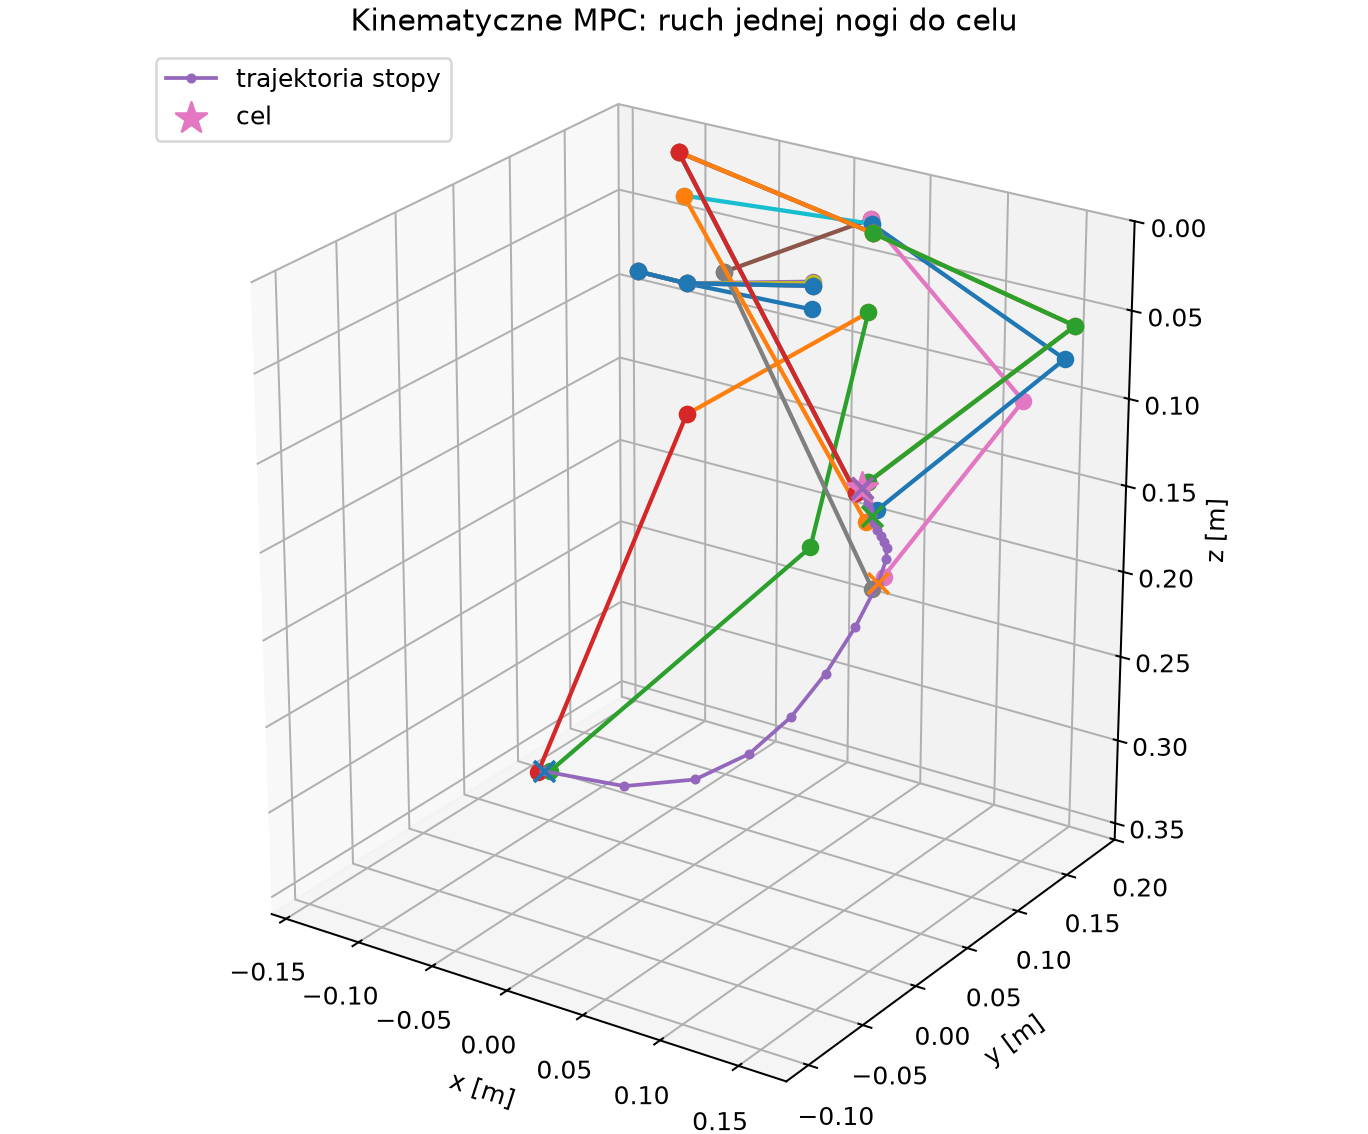
\includegraphics[width=\linewidth,height=0.55\textheight,keepaspectratio]{figures/mpc_leg_trajectory.png}
\end{columns}
\note{Należy uczciwie powiedzieć, że demonstrator steruje prędkościami przegubów. Model momentowy pojawia się dopiero jako następny etap projektu i w appendixie.}
\end{frame}

% 18
\begin{frame}{Funkcja kosztu i stan demonstratora}
\begin{columns}[T,onlytextwidth]
\column{0.52\textwidth}
\small
\[
\begin{aligned}
J ={}& w_p\|p_F-p_F^{\mathrm{ref}}\|^2
 + w_q\|q-q_{\mathrm{nom}}\|^2\\
&+ w_u\|\dot q\|^2
 + w_{\Delta u}\|\Delta\dot q\|^2.
\end{aligned}
\]
\begin{itemize}
  \item $w_p$: dokładność położenia stopy.
  \item $w_q$: preferowana, odzyskiwalna postawa.
  \item $w_u$: umiarkowane prędkości napędów.
  \item $w_{\Delta u}$: płynne zmiany sterowania.
\end{itemize}
\column{0.44\textwidth}
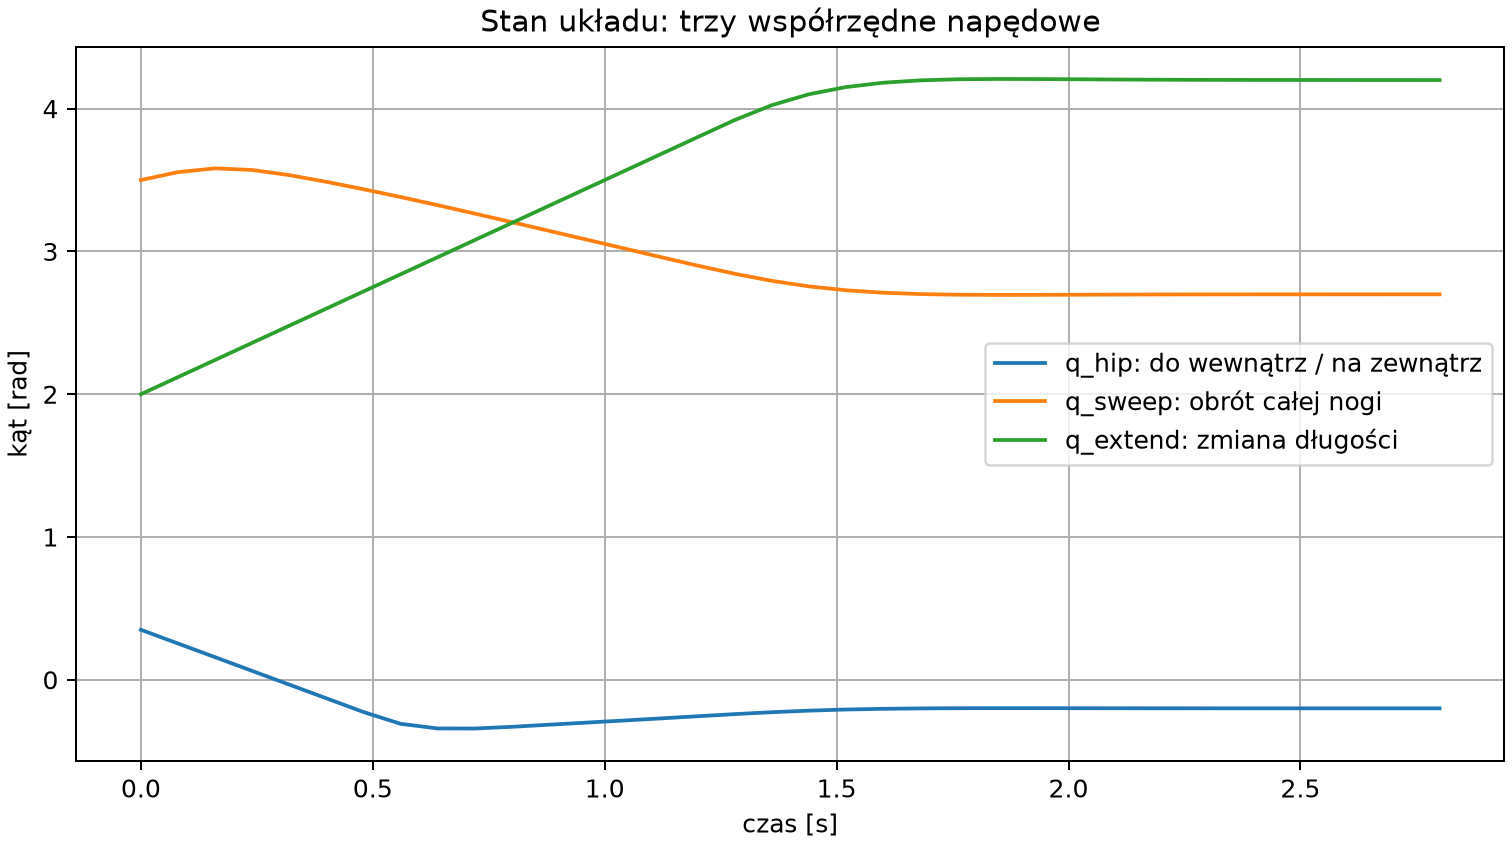
\includegraphics[width=\linewidth,height=0.50\textheight,keepaspectratio]{figures/mpc_joint_states.png}
\end{columns}
\begin{block}{Następny poziom}
Po identyfikacji dynamiki wejście $u=\dot q$ można zastąpić momentem $u=\tau$.
\end{block}
\note{Ten slajd usuwa niespójność między kodem a wcześniejszą wersją prezentacji, która opisywała od razu regulator momentowy.}
\end{frame}

% 19
\begin{frame}{Ograniczenia są sednem demonstratora}
\begin{columns}[T,onlytextwidth]
\column{0.48\textwidth}
\begin{block}{Ograniczenia modelu kinematycznego}
\[
q_{\min}\le q\le q_{\max},
\qquad
|\dot q|\le \dot q_{\max}
\]
\[
h_{\mathrm{spread}}(q)\ge 0,
\qquad
h_{\mathrm{toggle}}(q)\ge 0.
\]
\end{block}
\small
Marginesy są jawne, lecz na tym etapie pozostają heurystykami demonstracyjnymi.
\column{0.48\textwidth}
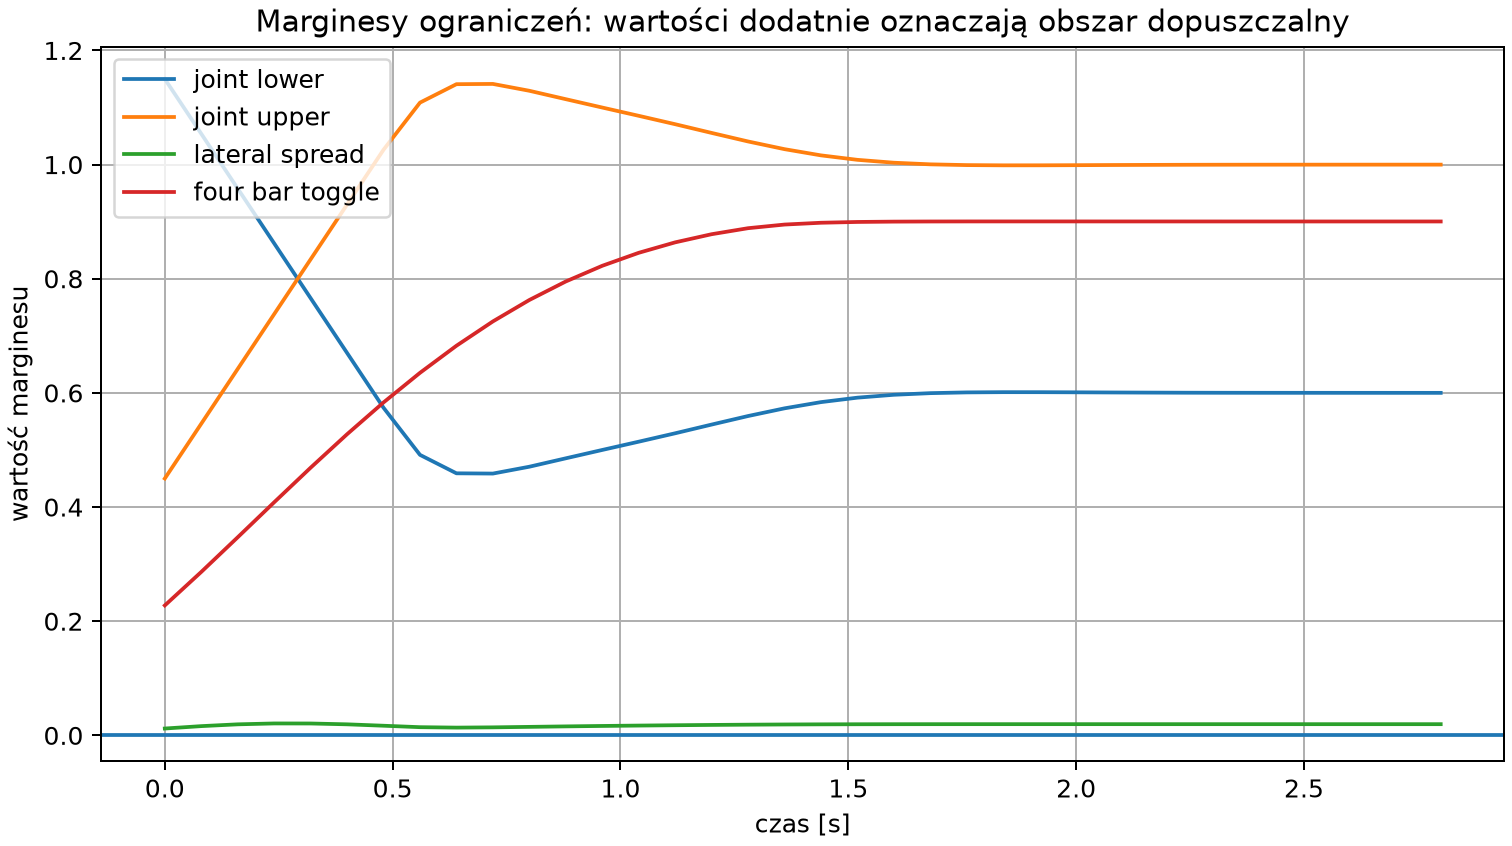
\includegraphics[width=\linewidth,height=0.50\textheight,keepaspectratio]{figures/mpc_safety_margins.png}
\end{columns}
\begin{block}{Docelowo}
Dodać moment, tarcie, kontakt i odzyskiwalność, a następnie sformułować warunki barierowe.
\end{block}
\note{Nie należy nazywać obecnych marginesów formalnymi gwarancjami. Ich wartość polega na tym, że tworzą mierzalny interfejs do przyszłych CBF i testów sprzętowych.}
\end{frame}

% 20
\begin{frame}{Rodzaje MPC używane w lokomocji}
\small
\begin{tabular}{p{0.29\textwidth}p{0.31\textwidth}p{0.30\textwidth}}
\toprule
\textbf{Rodzaj} & \textbf{Co upraszcza?} & \textbf{Po co?}\\
\midrule
Liniowe / wypukłe MPC & linearyzacja modelu, wypukłe ograniczenia & szybkie rozwiązywanie, prosty model\\[0.25em]
\midrule
Nieliniowe MPC & mniej uproszczeń w dynamice & lepsza dokładność, większy koszt obliczeń\\[0.25em]
\midrule
Centroidalne MPC & skupienie na środku masy i momencie pędu & dobre dla kontaktów i~równowagi\\[0.25em]
\midrule
MPC całego ciała & wszystkie przeguby i pełniejszy model & mniej warstw pośrednich, trudniejsze obliczenia\\[0.25em]
\midrule
MPC próbkowane & wiele kandydatów trajektorii & łatwe do zrównoleglenia, czasem mniej eleganckie matematycznie\\
\bottomrule
\end{tabular}
\source{Klasyczny przykład szybkiego wypukłego MPC: MIT Cheetah 3, Di Carlo i wsp., IROS 2018.}
\note{Użytkownik chciał zostawić ten slajd przed WBC i SRB. Należy tu podkreślić, że nie ma jednego „MPC”. Rodzina metod różni się modelem, solverem i miejscem w architekturze.}
\end{frame}

% 21
\begin{frame}{Chód jako harmonogram kontaktów}
\begin{columns}[T,onlytextwidth]
\column{0.48\textwidth}
\begin{itemize}
  \item Chód robota można opisać jako informację: która stopa dotyka podłoża w danym czasie.
  \item Harmonogram kontaktów decyduje, jakie siły wolno planować.
  \item Dla czworonoga typowe wzorce to stęp, kłus, galop, ale projekt badawczy może zacząć od prostszych sekwencji.
\end{itemize}
\column{0.48\textwidth}
\begin{center}
\begin{tikzpicture}[x=0.62cm,y=0.55cm]
  \foreach \r/\name in {0/FL,1/FR,2/RL,3/RR} {
    \node[font=\scriptsize] at (-0.6,-\r) {\name};
    \foreach \t in {0,...,7} {
      \pgfmathtruncatemacro{\contact}{mod(\t+\r,2)}
      \ifnum\contact=0
        \fill[safe!80] (\t,-\r) rectangle +(0.82,0.34);
      \else
        \fill[black!12] (\t,-\r) rectangle +(0.82,0.34);
      \fi
    }
  }
  \node[font=\scriptsize] at (3.4,-4.0) {zielone: kontakt, szare: przenoszenie};
\end{tikzpicture}
\end{center}
\end{columns}
\begin{block}{Rola MPC}
Dla zadanego harmonogramu kontaktów sterowanie predykcyjne dobiera ruch i siły tak, aby ciało pozostało stabilne i wykonalne.
\end{block}
\note{Tu można ostrożnie powiedzieć, że w pierwszym etapie harmonogram może być zadany z góry. Dopiero później można optymalizować także wybór kontaktów.}
\end{frame}

% 22
\begin{frame}{MPC dla humanoidów i psów: podobieństwa i różnice}
\scriptsize
\begin{tabular}{p{0.23\textwidth}p{0.32\textwidth}p{0.32\textwidth}}
\toprule
 & \textbf{Czworonóg} & \textbf{Humanoid}\\
\midrule
Kontakty & większa redundancja, więcej nóg w podporze & mniejszy wielokąt podparcia, częściej krytyczna równowaga\\[0.25em]
Priorytet & teren, odporność, sekwencje kontaktów & równowaga, manipulacja, koordynacja całego ciała\\[0.25em]
Model & często Single Rigid Body i siły kontaktu & często model centroidalny lub całego ciała\\[0.25em]
Ryzyko & poślizg, zahaczenie, złe ułożenie nogi & upadek, kontakt nieplanowany, sprzężenie z manipulacją\\
\bottomrule
\end{tabular}
\vspace{0.6em}
\begin{block}{Dlaczego to ważne dla projektu?}
\small Czworonóg jest praktycznym poligonem testowym dla idei potrzebnych także w~robocie humanoidalnym: kontaktu, predykcji, ograniczeń i bezpieczeństwa.
\end{block}
\note{Slajd powinien uspokoić odbiorców, że praca na czworonogu nie jest ślepą uliczką. To dobry testbed dla metod, które później skalują się do humanoidów.}
\end{frame}

% 23
\begin{frame}{Single Rigid Body: model pojedynczego ciała sztywnego}
\begin{block}{Single Rigid Body (SRB)}
Model pojedynczego ciała sztywnego traktuje korpus robota jako jedno ciało, a nogi głównie jako źródła sił kontaktowych.
\end{block}
\begin{columns}[T,onlytextwidth]
\column{0.48\textwidth}
\begin{itemize}
  \item Plus: prostszy, szybki, użyteczny dla planowania sił reakcji podłoża.
  \item Plus: popularny w czworonożnej lokomocji dynamicznej.
\end{itemize}
\column{0.48\textwidth}
\begin{itemize}
  \item Minus: pomija dużą część dynamiki nóg.
  \item Minus: nietypowa noga z mechanizmem czworoboku może wymagać dodatkowych ograniczeń niżej w sterowaniu.
\end{itemize}
\end{columns}
\source{Praktyczne implementacje SRB/MPC są dostępne np. w Quadruped-PyMPC.}
\note{Przy pierwszym użyciu podajemy pełną nazwę i dopiero potem skrót. Ważne: SRB nie rozwiąże automatycznie problemu rozstawionej nogi, bo może w ogóle nie widzieć szczegółów mechanizmu.}
\end{frame}

% 24
\begin{frame}{Whole-Body Control: sterowanie całym ciałem}
\begin{block}{Whole-Body Control (WBC)}
Sterowanie całym ciałem przekształca cele dla korpusu, stóp i sił kontaktowych na ruch lub momenty wszystkich przegubów.
\end{block}
\begin{center}
\begin{tikzpicture}[node distance=0.9cm,>=Latex]
  \tikzstyle{box}=[draw,rounded corners=2pt,fill=blue!6,minimum width=3.0cm,minimum height=0.72cm,align=center,font=\small]
  \node[box] (mpc) {Model Predictive\\Control};
  \node[box,right=of mpc] (wbc) {Whole-Body\\Control};
  \node[box,right=of wbc] (imp) {sterowanie\\impedancyjne};
  \node[box,right=of imp] (robot) {robot};
  \draw[->,thick] (mpc)--(wbc);
  \draw[->,thick] (wbc)--(imp);
  \draw[->,thick] (imp)--(robot);
\end{tikzpicture}
\end{center}
\begin{itemize}
  \item WBC może egzekwować zadania priorytetowe: kontakt, postawa, limity momentu, stabilizacja korpusu.
  \item Nowsze prace pokazują też MPC całego ciała z pełniejszą dynamiką, np. z MuJoCo.
\end{itemize}
\note{To powinien być slajd „gdzie to się wpina”. MPC może planować, WBC może realizować plan na wszystkich przegubach, a napędy mogą wykonywać warstwę impedancyjną.}
\end{frame}

% 25
\begin{frame}{Control Barrier Functions: funkcje barierowe bezpieczeństwa}
\begin{block}{Control Barrier Functions (CBF)}
Funkcje barierowe bezpieczeństwa opisują zbiór stanów dopuszczalnych i narzucają warunek, aby sterowanie nie wypchnęło układu poza ten zbiór.
\end{block}
\begin{columns}[T,onlytextwidth]
\column{0.48\textwidth}
\[
\mathcal C = \{x: h(x)\ge 0\}
\]
\[
\text{chcemy utrzymać } x(t)\in\mathcal C
\]
\column{0.48\textwidth}
\begin{itemize}
  \item $h(x)>0$: zapas bezpieczeństwa.
  \item $h(x)=0$: granica bezpieczeństwa.
  \item $h(x)<0$: stan narusza warunek.
\end{itemize}
\end{columns}
\begin{block}{Interpretacja dla nogi}
CBF nie musi uczyć chodu. Ma zabronić sterowania, które prowadzi w konfiguracje zbyt szerokie, osobliwe albo bez zapasu momentu.
\end{block}
\note{Należy użyć pełnej nazwy przed skrótem. Warto powiedzieć, że CBF to język do opisu bezpieczeństwa, a nie magiczna gwarancja bez dobrze zdefiniowanego modelu i zbioru bezpiecznego.}
\end{frame}

% 26
\begin{frame}{CBF jako filtr dla polityki uczonej}
\begin{columns}[T,onlytextwidth]
\column{0.54\textwidth}
\begin{center}
\begin{tikzpicture}[node distance=0.65cm,>=Latex]
  \tikzstyle{box}=[draw,rounded corners=2pt,fill=blue!6,minimum width=3.1cm,minimum height=0.75cm,align=center,font=\small]
  \node[box] (rl) {polityka Reinforcement\\Learning};
  \node[box,below=of rl] (filter) {filtr CBF / MPC};
  \node[box,below=of filter] (drive) {sterowanie napędów};
  \node[box,below=of drive] (robot) {robot + podłoże};
  \draw[->,thick] (rl)--node[right,font=\scriptsize]{propozycja} (filter);
  \draw[->,thick] (filter)--node[right,font=\scriptsize]{bezpieczna korekta} (drive);
  \draw[->,thick] (drive)--(robot);
  \draw[->,thick] (robot.west) .. controls +(-1.2,0) and +(-1.2,0) .. (filter.west);
\end{tikzpicture}
\end{center}
\column{0.42\textwidth}
\begin{itemize}
  \item RL proponuje szybkie zachowanie.
  \item Filtr sprawdza warunki bezpieczeństwa.
  \item Jeśli akcja jest ryzykowna, filtr ją koryguje lub odrzuca.
\end{itemize}
\begin{block}{Najbliższa literatura}
CBF + MPC zademonstrowano m.in. na ANYmalu w pracy o wielowarstwowym bezpieczeństwie lokomocji.
\end{block}
\end{columns}
\note{To slajd z bardzo praktycznym przekazem: nie trzeba od razu zastępować RL. Można zacząć od nadzorcy, który ma jawny model i jawne bariery.}
\end{frame}

% 27
\begin{frame}{Docelowa architektura projektu}
\begin{center}
\begin{tikzpicture}[node distance=0.45cm and 0.42cm,>=Latex]
  \tikzstyle{box}=[draw,rounded corners=2pt,fill=blue!6,minimum width=1.95cm,minimum height=0.62cm,align=center,font=\scriptsize]
  \node[box] (sensors) {czujniki};
  \node[box,right=of sensors] (est) {estymacja\\stanu};
  \node[box,right=of est] (rl) {polityka\\RL};
  \node[box,right=of rl] (mpc) {MPC / filtr\\bezpieczeństwa};
  \node[box,right=of mpc] (drive) {sterowanie\\impedancyjne};
  \node[box,right=of drive] (robot) {robot};
  \node[box,below=of mpc] (cbf) {warstwa CBF};
  \draw[->,thick] (sensors)--(est);
  \draw[->,thick] (est)--(rl);
  \draw[->,thick] (rl)--(mpc);
  \draw[->,thick] (cbf)--(mpc);
  \draw[->,thick] (mpc)--(drive);
  \draw[->,thick] (drive)--(robot);
  \draw[->,thick] (est.south) |- (cbf.west);
  \draw[->,thick] (robot.south) .. controls +(0,-0.9) and +(0,-0.9) .. (sensors.south);
\end{tikzpicture}
\end{center}
\vspace{0.2em}
\begin{itemize}
  \item Wersja minimalna: CBF/MPC filtruje ryzykowne konfiguracje jednej nogi.
  \item Wersja rozszerzona: MPC planuje siły kontaktowe, a WBC rozdziela zadania na przeguby.
  \item Warunek projektu naukowego: mierzalna redukcja awarii poza scenariuszami treningowymi.
\end{itemize}
\note{To jest slajd spinający projekt. Można na nim powiedzieć: nie budujemy wszystkiego naraz. Pierwszy etap to mały filtr bezpieczeństwa i model jednej nogi, dopiero później pełna lokomocja.}
\end{frame}

% 28
\begin{frame}{Demonstracja czy wynik badawczy?}
\begin{columns}[T,onlytextwidth]
\column{0.48\textwidth}
\begin{block}{Demonstracja}
\begin{itemize}
  \item Robot przeszedł trasę.
  \item Film wygląda przekonująco.
  \item Sukces może zależeć od jednego podłoża, jednej baterii i jednego strojenia.
\end{itemize}
\end{block}
\column{0.48\textwidth}
\begin{block}{Wynik badawczy}
\begin{itemize}
  \item Zdefiniowano klasę awarii.
  \item Metoda mierzalnie redukuje tę klasę awarii.
  \item Testy obejmują podłoża, zakłócenia i przypadki spoza treningu.
\end{itemize}
\end{block}
\end{columns}
\vspace{0.4em}
\begin{block}{Proponowane kryterium pierwszego etapu}
Na jednej nodze: mniej wejść w konfiguracje nieodzyskiwalne przy ograniczeniach tarcia, momentu i geometrii, bez utraty zdolności do osiągania punktów roboczych.
\end{block}
\note{Użytkownik chciał mocniej podkreślić różnicę między projektem demonstracyjnym i naukowym. Tu jest sedno: film nie wystarcza. Trzeba mieć definicję awarii, metrykę i porównanie z bazą.}
\end{frame}

% 29 Appendix A
\appendix
\begin{frame}{Appendix A: od sił kontaktowych do momentów napędów}
\begin{columns}[T,onlytextwidth]
\column{0.48\textwidth}
\begin{block}{Najprostsza intuicja statyczna}
\[
\tau \approx J(q)^T f
\]
\end{block}
\begin{itemize}
  \item $f$ - siła działająca w stopie.
  \item $J(q)^T$ - przeniesienie siły na momenty przegubów.
\end{itemize}
\column{0.48\textwidth}
\begin{block}{W rzeczywistości dochodzi}
\begin{itemize}
  \item dynamika członów,
  \item więzy mechanizmu równoległego,
  \item tarcie i poślizg,
  \item limity napędów i przekładni,
  \item opóźnienia komunikacji i regulatorów.
\end{itemize}
\end{block}
\end{columns}
\begin{block}{Dlaczego appendix?}
Ten slajd jest dobry do dyskusji technicznej, ale nie jest potrzebny każdemu odbiorcy w głównej narracji.
\end{block}
\note{Appendix pomaga, jeśli ktoś zapyta: skąd momenty w silnikach biorą się z planowania sił kontaktowych. To też miejsce na dyskusję, czy model jednej nogi wystarczy.}
\end{frame}

% 30 Appendix B
\begin{frame}{Appendix B: materiały startowe i pełniejszy problem}
\small
\begin{itemize}
  \item \href{https://underactuated.mit.edu/trajopt.html}{MIT Underactuated Robotics: Trajectory Optimization} - najlepszy pierwszy materiał o optymalizacji trajektorii i idei przesuwającego się horyzontu.
  \item \href{https://ieeexplore.ieee.org/document/8594448}{MIT Cheetah 3 przez wypukłe MPC} - klasyczny przykład szybkiego planowania sił reakcji podłoża dla czworonoga.
  \item \href{https://github.com/iit-DLSLab/Quadruped-PyMPC}{Quadruped-PyMPC} - praktyczny kod w Pythonie dla MPC opartego o model pojedynczego ciała sztywnego.
  \item \href{https://arxiv.org/abs/2011.00032}{CBF + MPC dla ANYmal} - najbliższy punkt startowy dla warstwy bezpieczeństwa w robotach kroczących.
  \item \href{https://arxiv.org/abs/2503.04613}{Whole-Body MPC z MuJoCo} - współczesny przykład MPC całego ciała dla czworonogów i humanoidów.
\end{itemize}
\vspace{-0.25em}
\begin{block}{Pełniejsza formulacja jednej nogi}
\[
\min \sum_k \left(
\|p_F-p_F^{ref}\|^2 + \|q-q_{nom}\|^2 + \|\tau\|^2\right)
\]
\[
\Phi(q,z)=0,\quad q_{min}\le q\le q_{max},\quad |\tau|\le\tau_{max},\quad h(q,\dot q)\ge0.
\]
\end{block}
\note{To jest slajd kończący i jednocześnie źródła. Każdy materiał ma jedno zdanie opisu, tak jak użytkownik poprosił. Dyad jest świadomie pominięty ze względu na komercyjną licencję, a może być wspomniany ustnie.}
\end{frame}


\end{document}
